\documentclass[epsfig]{article}
\usepackage{epsfig}
\usepackage{amsmath}
\usepackage{verbatim}
\usepackage{booktabs}
\usepackage{subfig}
\usepackage{graphicx}
\usepackage{diagbox} 
\usepackage{tabularx}
\usepackage[english]{babel}
\usepackage{float}
\textwidth 6.7in
\oddsidemargin -0.1in
\textheight 8.50in
\topmargin -0.55in
\renewcommand{\textfraction}{0.25}
\renewcommand{\floatpagefraction}{0.7}
\markboth{}{\sl E. Mer\'enyi \hfil COMP / ELEC / STAT 502 \hfil Homework 4 }
\pagestyle{myheadings}
\def\bpar{\vskip26pt}
\def\npar{\vskip13pt}
\def\spar{\vskip10pt}
\begin{document}
\parindent=0pt
\null
{\bf 
	\npar
	Problem 1
	\bpar
}
\begin{table}[htbp] 
\center
\caption{Parameters of Training BP Network to Fit Iris data}

%\scalebox{0.9}{ % You can scale the size of the table by changing this number
\scalebox{1.0}{
	\begin{tabular}{p{4cm} p{.05cm} p{8cm}}
		\toprule
		\multicolumn{3}{l}{\bf Network parameters} \\
		\bottomrule \noalign{\smallskip}
		Topology & & $(4 + 1_{Bias})$ --- $(2+1_{Bias} )$ --- $3$ \\
		Transfer function & & tanh with slope of 1 \\
		\toprule
		\multicolumn{3}{l}{\bf Learning parameters} \\
		\bottomrule \noalign{\smallskip}
		Initial weights & & drawn from U[$-1\over{\sqrt{NPE}}$,$1\over{\sqrt{NPE}}$] \\
		Learning rate ($\alpha$) & & 0.01 \\
		Momentum & & 0.7\\
		Epoch size ($Epoch$)& &  100 \\
		Stopping criteria & & RMSE$ < 0.2$ or  learn count (t) $ > 500 \times 100 $\\
		Error measure & &$1-{{Number\ of\ CorrectlyClassified\ Inputs}\over{Number \ of\ All\ Inputs}}$(1-Accurancy) and RMSE \\\toprule
		\multicolumn{3}{l}{\bf Input / output data, representation, scaling} \\
		\bottomrule \noalign{\smallskip}
		\# training samples ($N_{tr}$)& & 100 \\
		\# test samples ($N_{tst}$)& & 50 \\
		Scaling of inputs & &  already scaled \\
		Scaling of outputs & &  set the maximum element of each column to 1, others to 0  \\
		
		\bottomrule \noalign{\smallskip}
		
	\end{tabular}
} % end scalebox
\end{table}





\begin{figure}[H]
	\caption{Training and Test Accurancy for Each Fold}
	\begin{minipage}[t]{0.3\linewidth}
		\centering
		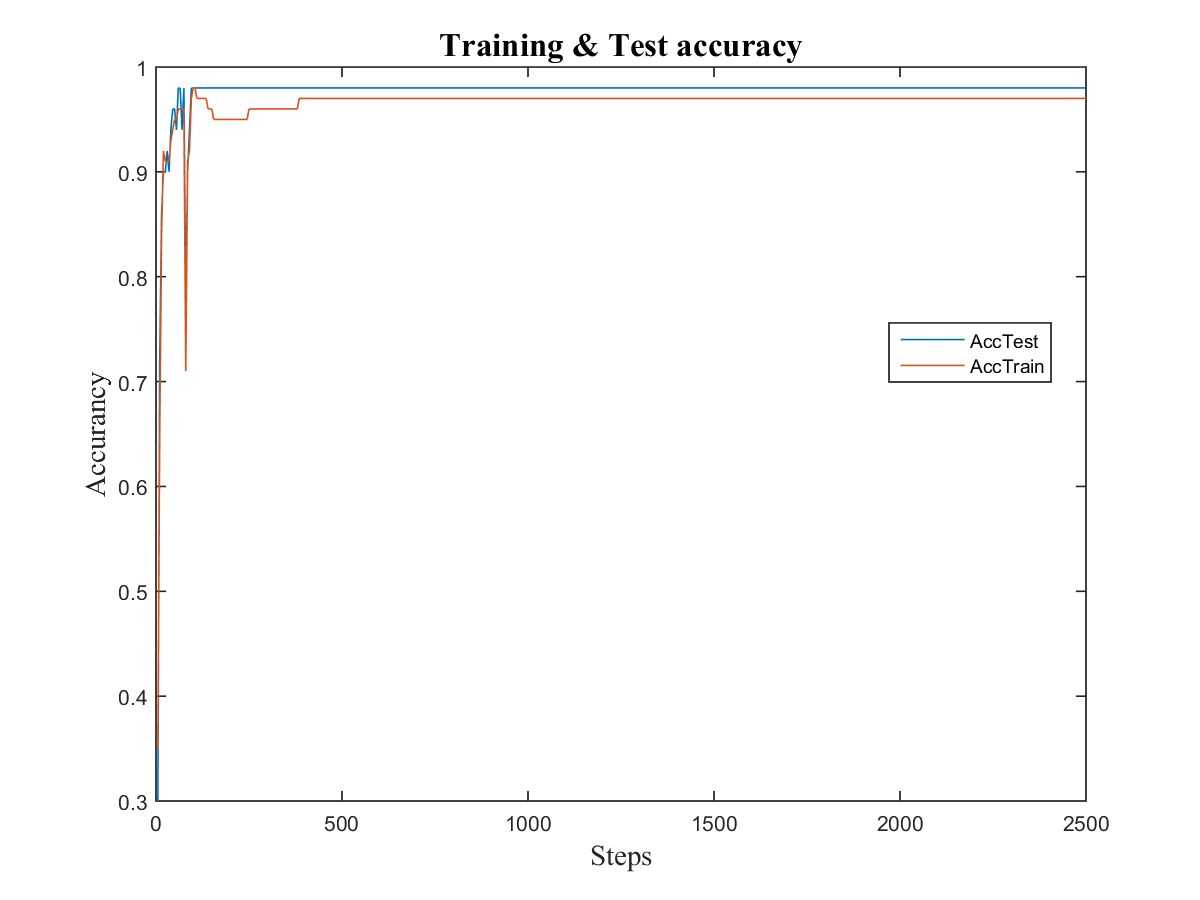
\includegraphics[width=2.2in]{Acc_1.png}


	\end{minipage}%
	\begin{minipage}[t]{0.3\linewidth}
		\centering
		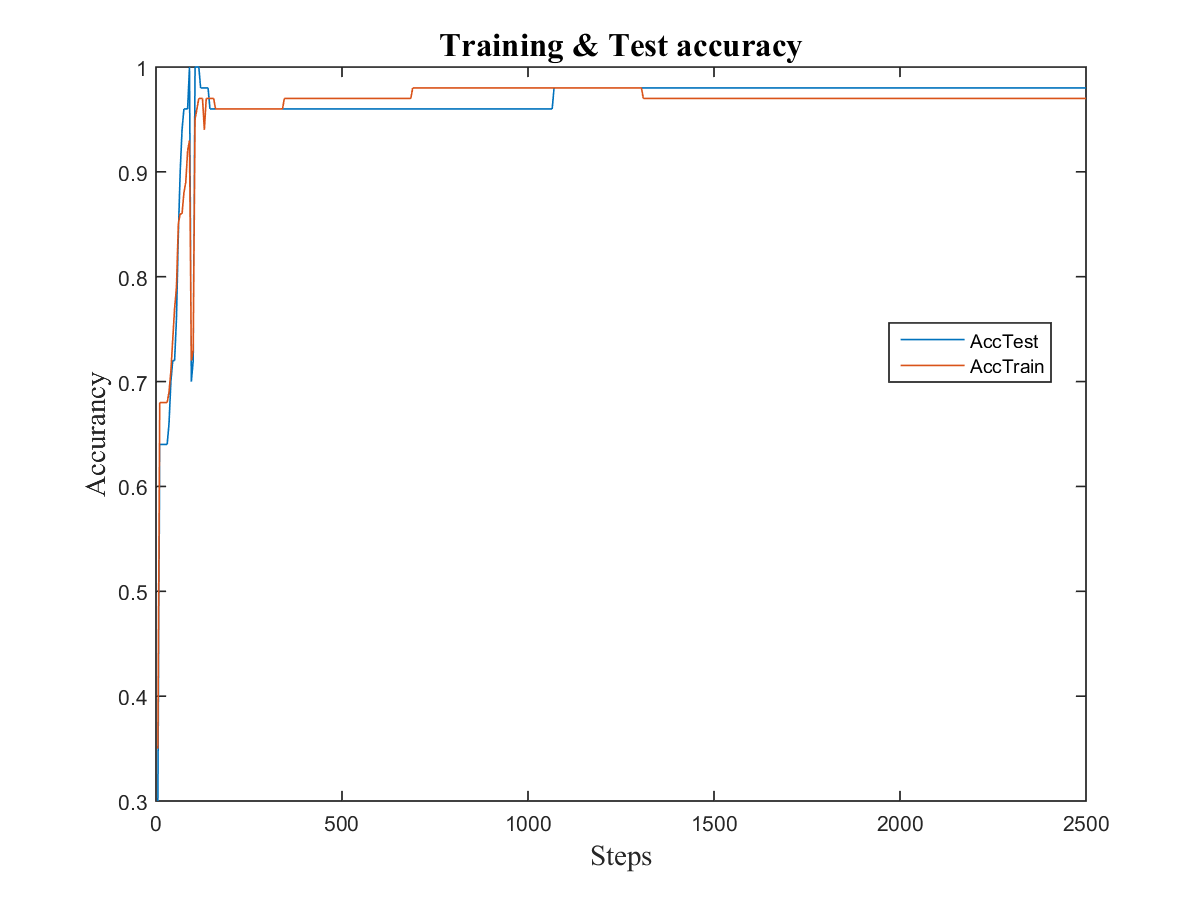
\includegraphics[width=2.2in]{Acc_2.png}


	\end{minipage}
	\begin{minipage}[t]{0.3\linewidth}
	\centering
	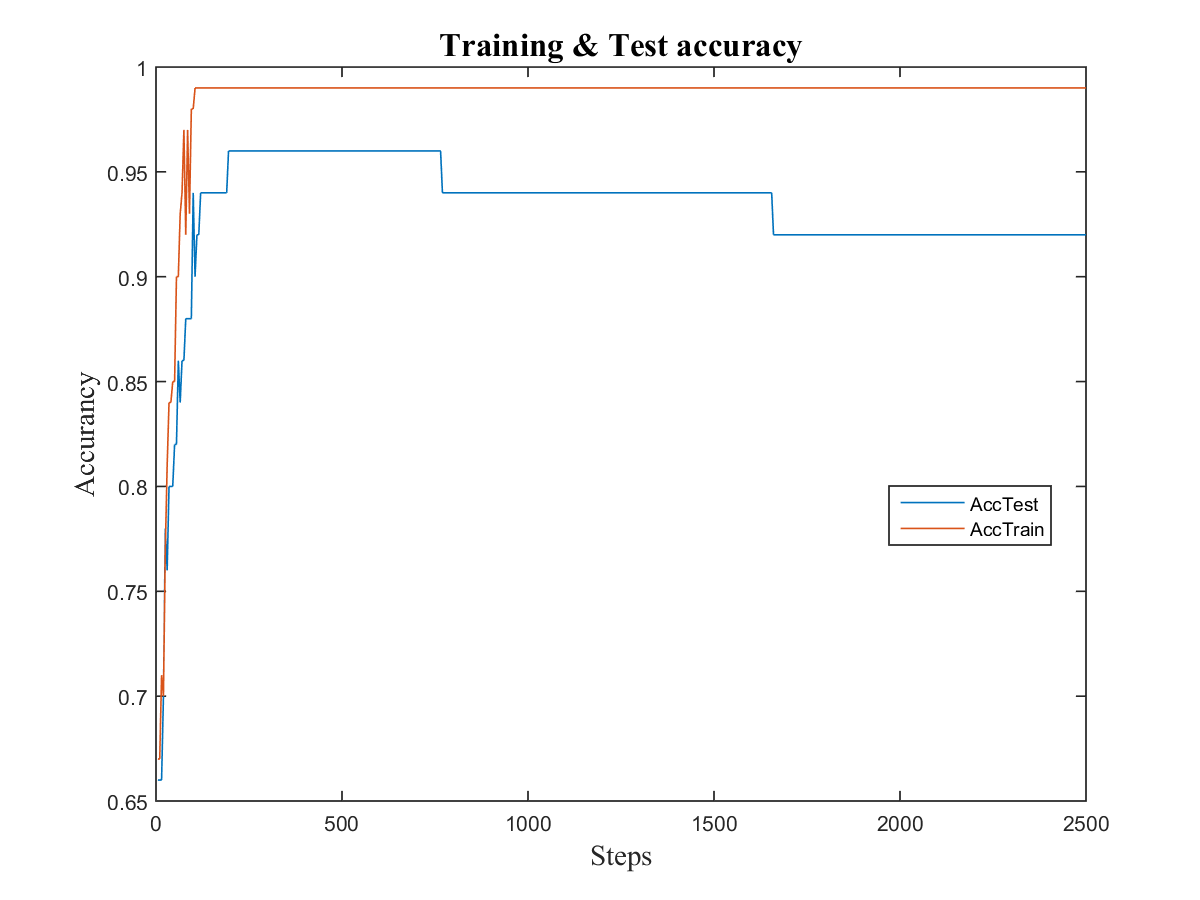
\includegraphics[width=2.2in]{Acc_3.png}


\end{minipage}
\end{figure}

\begin{figure}[H]
	\caption{Training and Test RMSE for Each Fold}
	\begin{minipage}[t]{0.3\linewidth}
		\centering
		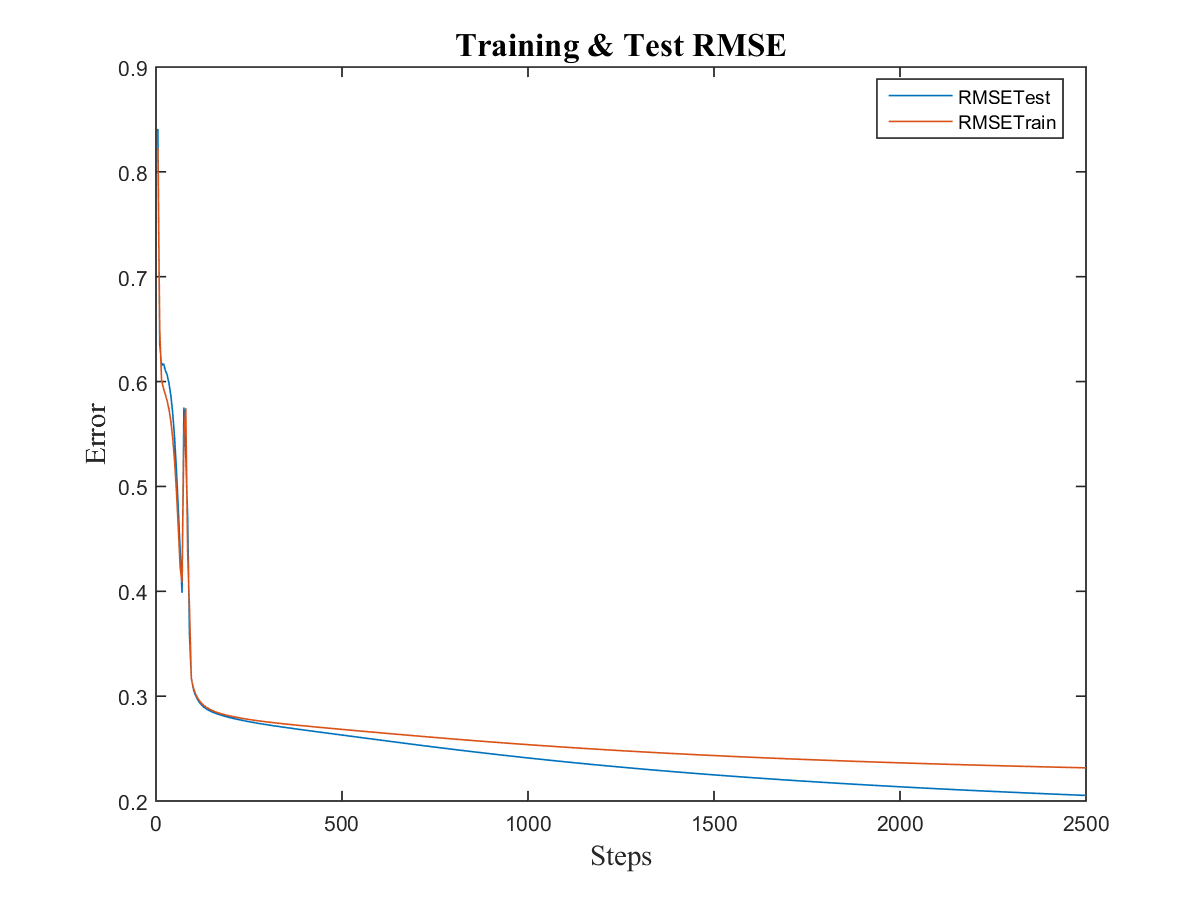
\includegraphics[width=2.2in]{RMSE_1.png}
		
		
	\end{minipage}%
	\begin{minipage}[t]{0.3\linewidth}
		\centering
		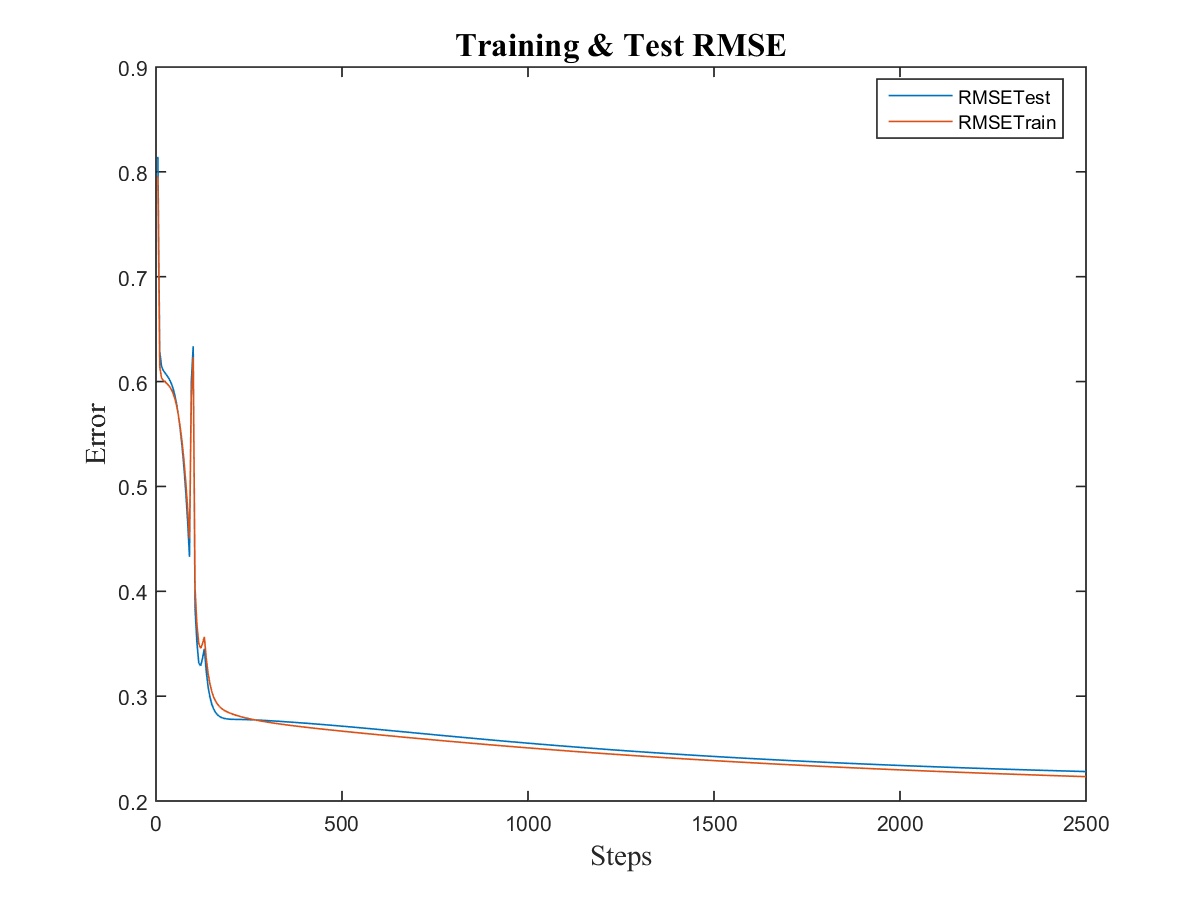
\includegraphics[width=2.2in]{RMSE_2.png}
		
		
	\end{minipage}
	\begin{minipage}[t]{0.3\linewidth}
		\centering
		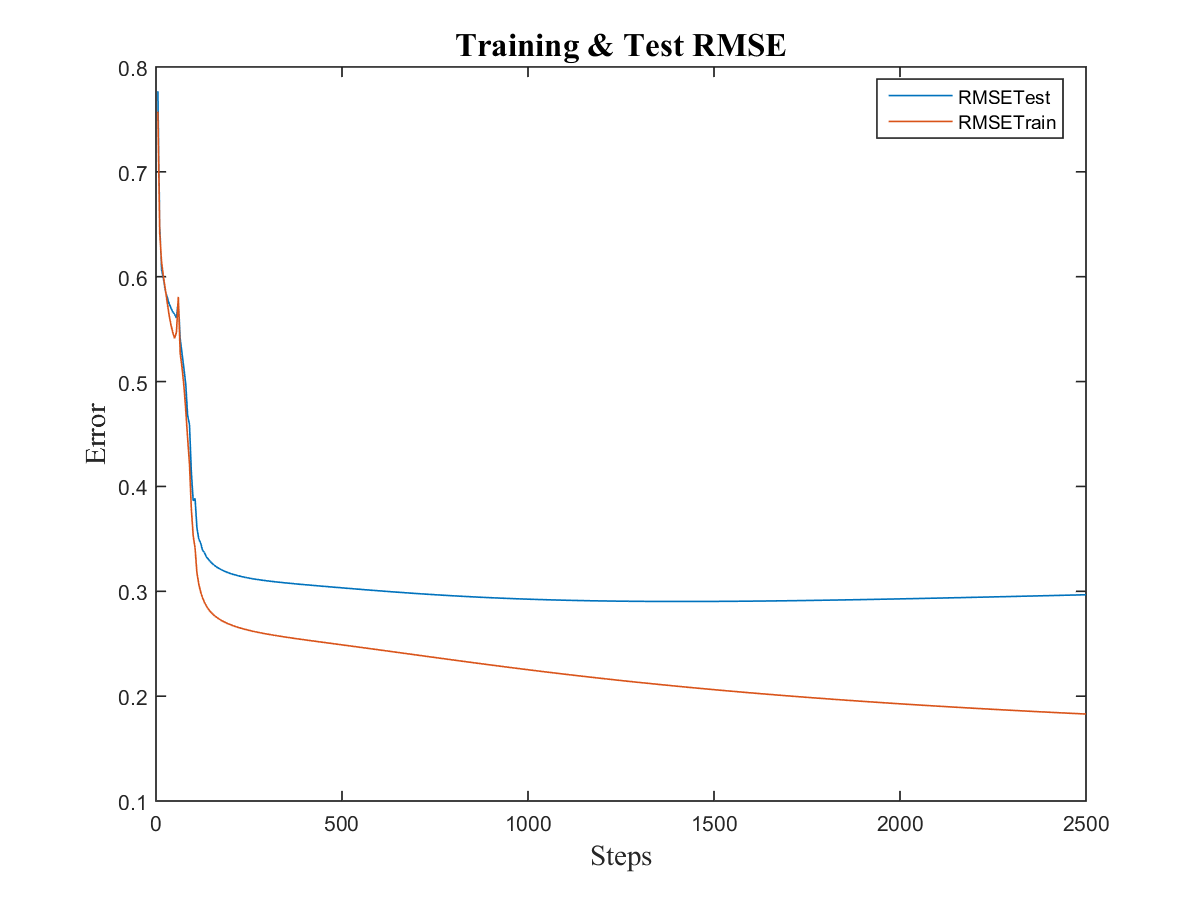
\includegraphics[width=2.2in]{RMSE_3.png}
		
		
	\end{minipage}
\end{figure}

This time we used same parameters (except epoch  size) as HW4. For cross-validation, all the data is randomly splited into 3 sets. For each fold one of these sets is used as test set, and other sets are merged and used as training set. Then we perform training and test on each fold seperately. \\
\\
In HW4 we had already used confusion matrix to display the result. This time we just used the same procedure and format. We can see that the performance of each fold is similar, which indicates that the network is well generalized.\\
\\
Note that I didn't give the "actual vs desired" plot. That's because I think the plot cannot give any information which is not given by confusion matrix, and is much more messive. In the text of HW5, it's said that the plot could show the "localization" of misclassified data, but this "localization" doesn't make any sense. The order of the data is trivial in the classification, furthermore, the order is rearranged in the cross validation. If we want to know the real "localization" of misclassifications, we need to see the INPUT of them, but we cannot plot that since the Input is 4-dimensional.\\

\begin{table}[H]
	\caption{Results of the cross validation(training set)}
	
	\begin{tabular}{|l|ccc|ccc|ccc|}
		\hline
		& &Fold 1 & & &Fold 2 & & &Fold 3 &\\
		\hline
		
		\diagbox{Actual}{Desired} & Class 1 & Class 2 & Class 3& Class 1 & Class 2 & Class 3& Class 1 & Class 2 & Class 3 \\
		\hline
		Class 1&35 &0 &0&33 &0 &0&32 &0 &0\\
		Class 2&0 & 34&2& 0&30 &1&0 &32 &0\\
		Class 3&0 &1 &28& 0&2 &34&0 &1 &35\\

		\hline
		Overall	Accurancy & &0.97 & & &0.97&  & &0.99 &  \\
		\hline
		
	\end{tabular}\spar
	Mean Accurancy of Each Fold: 0.978    \\
	Std of Accurancy: 0.0115
\end{table}
\begin{table}[H]
	\caption{Results of the cross validation(test set)}

	\begin{tabular}{|l|ccc|ccc|ccc|}
		\hline
		& &Fold 1 & & &Fold 2 & & &Fold 3 &\\
	\hline

	\diagbox{Actual}{Desired} & Class 1 & Class 2 & Class 3& Class 1 & Class 2 & Class 3& Class 1 & Class 2 & Class 3 \\
	\hline
	Class 1&15 &0 &0&17 &0 &0&18 &0 &0\\
	Class 2&0 & 14&0& 0&18 &1&0 &16 &3\\
	Class 3&0 &1 &20& 0&0 &14&0 &1 &12\\
	

		\hline
	Overall	Accurancy & &0.98 & & &0.98&  & &0.92 &  \\
	\hline

\end{tabular}\spar
			Mean Accurancy of Each Fold: 0.96    \\
			Std of Accurancy: 0.0346
\end{table}
			*Class 1 is Setosa, Class 2 is Versacolor, Class 3 is Virginica

{\bf 
\npar
Problem 2
\bpar
}


\begin{table}[htbp] 
\center
\caption{Parameters of Training BP Network to perform the equalization of the communication channel}
  \label{tab:NP}
  %\scalebox{0.9}{ % You can scale the size of the table by changing this number
   \scalebox{1.0}{
   \begin{tabular}{p{4cm} p{.05cm} p{8cm}}
\toprule
  \multicolumn{3}{l}{\bf Network parameters} \\
\bottomrule \noalign{\smallskip}
  Topology & & $(1 + 1_{Bias})$ --- $(10 + 1_{Bias})$ (otherwise notified) --- $1$ \\
  Transfer function & & tanh with slope of 1(hidden layer) or linear(output layer) \\
\toprule
  \multicolumn{3}{l}{\bf Learning parameters} \\
\bottomrule \noalign{\smallskip}
  Initial weights & & drawn from U[$-1\over{\sqrt{NPE}}$,$1\over{\sqrt{NPE}}$] \\
  Learning rate ($\alpha$) & & 0.01, otherwise notified\\
  Momentum & & 0.9\\
  Epoch size ($Epoch$)& &  20\\
  Stopping criteria & &  error ($Err_{MSE}$) $<$ 0.0001 or learn steps =60,000\\
  Monitoring frequency of error measure & &  Every 1000 learn steps\\
  Error measure($Err_{MSE}$) & &  The sum of $(D-y)^2$ that averaged over all training or testing samples\\\toprule
 \multicolumn{3}{l}{\bf Input / output data, representation, scaling} \\
\bottomrule \noalign{\smallskip}
  \ Training samples ($S{(n)}$)& & $2sin({2\pi n \over 20}) $, $n$=1:20\\ 
    \ Test sample set 1 ($s_1{(n)}$)& &$0.8sin({2\pi n \over 10}) + 0.25cos({2\pi n \over 25})$,n=1:50\\
    \ Test sample set 2 ($s_2{(n)}$)& & 50 random numbers drawn from a zero mean, unit variance normal distribution\\
  Scaling & & none\\
  
 \bottomrule \noalign{\smallskip}
 
  \end{tabular}
   } % end scalebox
\end{table}


For all the output verses desired output plots, we used z(nT) as input(x axis), and $\hat{s}$(nT), s(nT) as output(y axis). \\
It's widely accepted that when doing regression, use linear output layer could achieve better performance. So this time we didn't scale the data, and use a linear transfer function in output layer correspondingly. \\
In this problem, we only care the performance of the neural network, so we just use the input and output to display the result, instead of the "original signal".\\


{\bf 
\npar
2.1) Training
\bpar
}
 

The MSE history is shown below:

\begin{figure}[H] 
\centering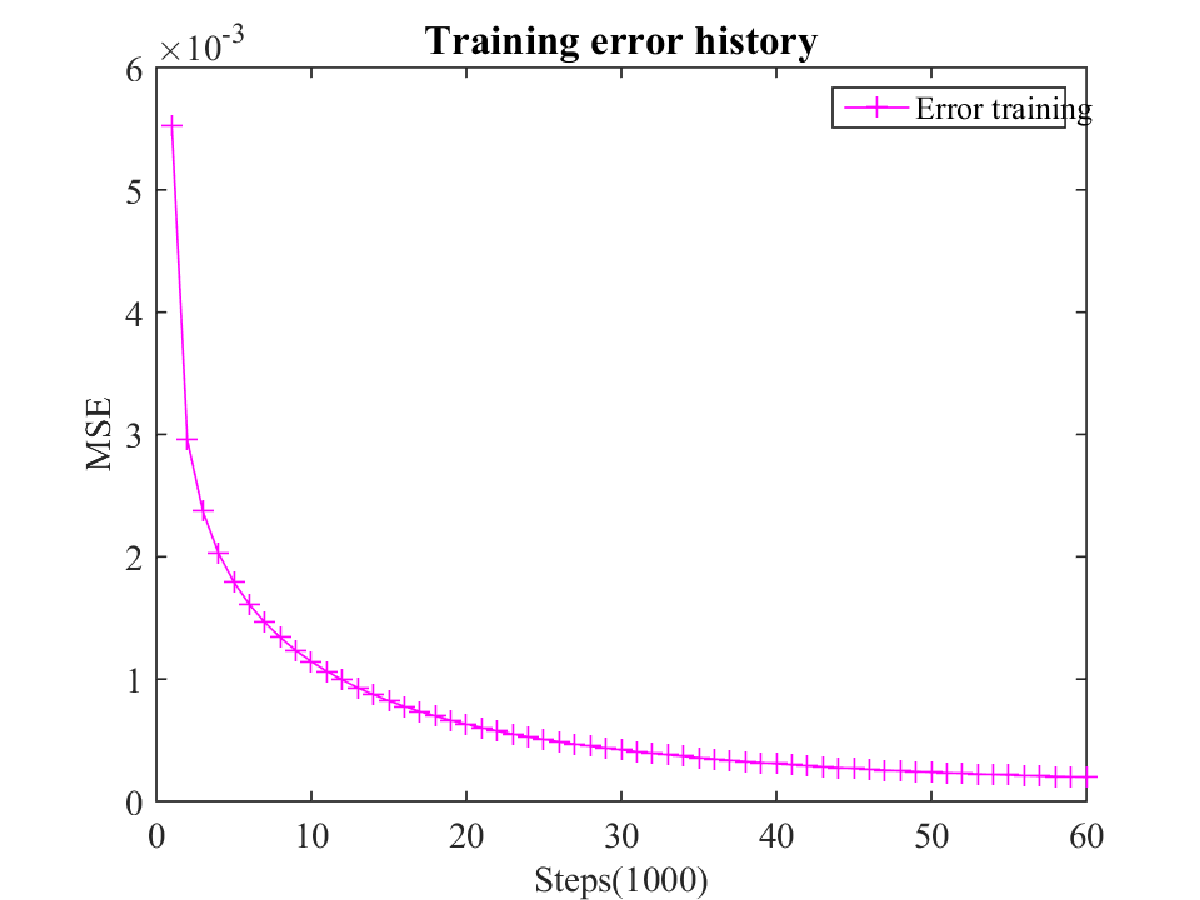
\includegraphics[width=4in]{MSEhistory_1.png} 
\end{figure} 

The training output versus desired output is shown as figure below.

\begin{figure}[H] 
\centering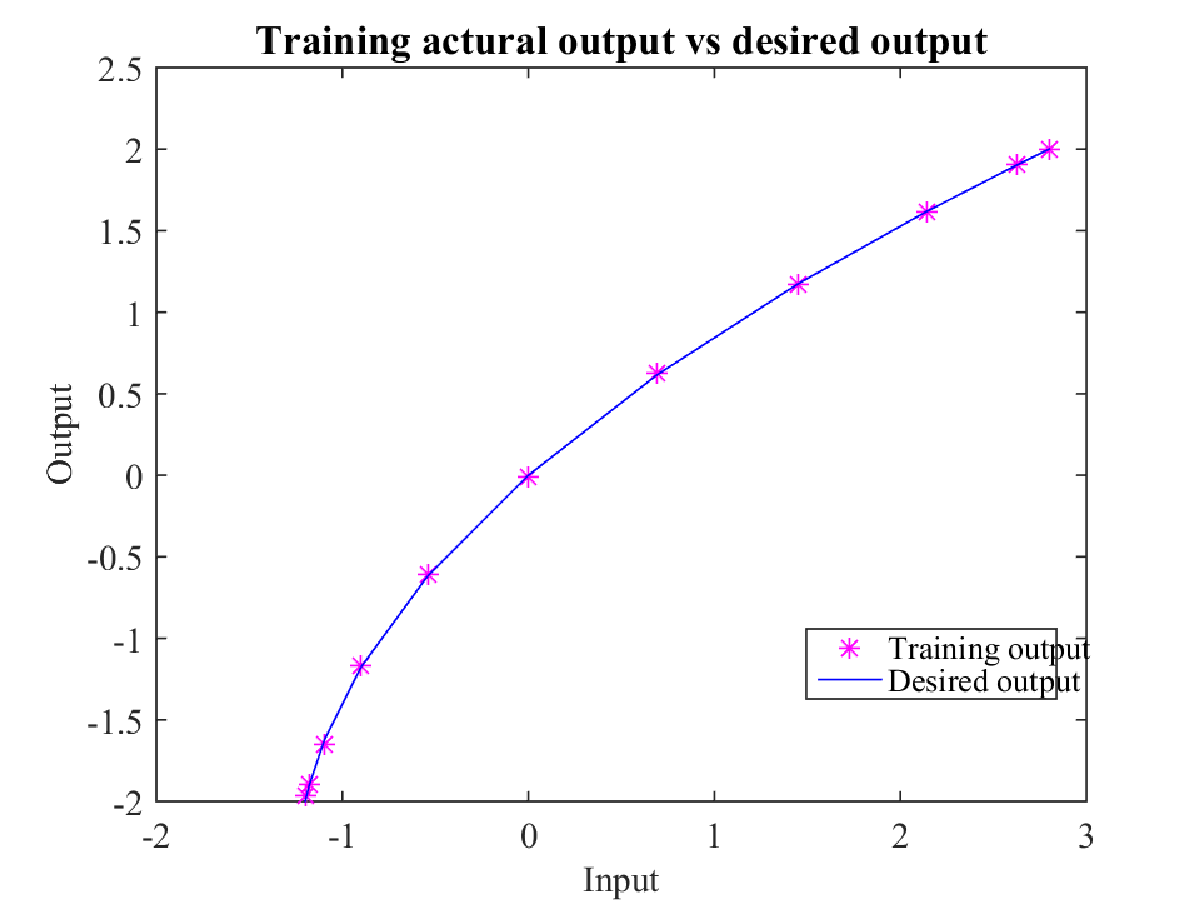
\includegraphics[width=4in]{TrainvsDesire_1.png} 
\end{figure} 


{\bf 
\npar
2.1.1) Different hidden PE number
\bpar
}

We first tried to use different number of hidden PE. By comparing the history, increasing the number of hidden PE did not significantly change the reduction of MSE, except for $\#$PE=1. For $\#$PE=1, it took longer time to reduce the MSE. The final error rate for $\#$PE=1, $\#$PE=5, $\#$PE=10, $\#$PE=80 are 0.0004, 0.0003, 0.0006, 0.0009. We noticed that the final MSE varied during repeating the training, so these values can only show that their final result were qualitatively the same.

In this case, the final output of training were almost overlapped to $\#$PE=10, so the training data vs desired data for each condition is not shown here.

\begin{figure}[H] 
\centering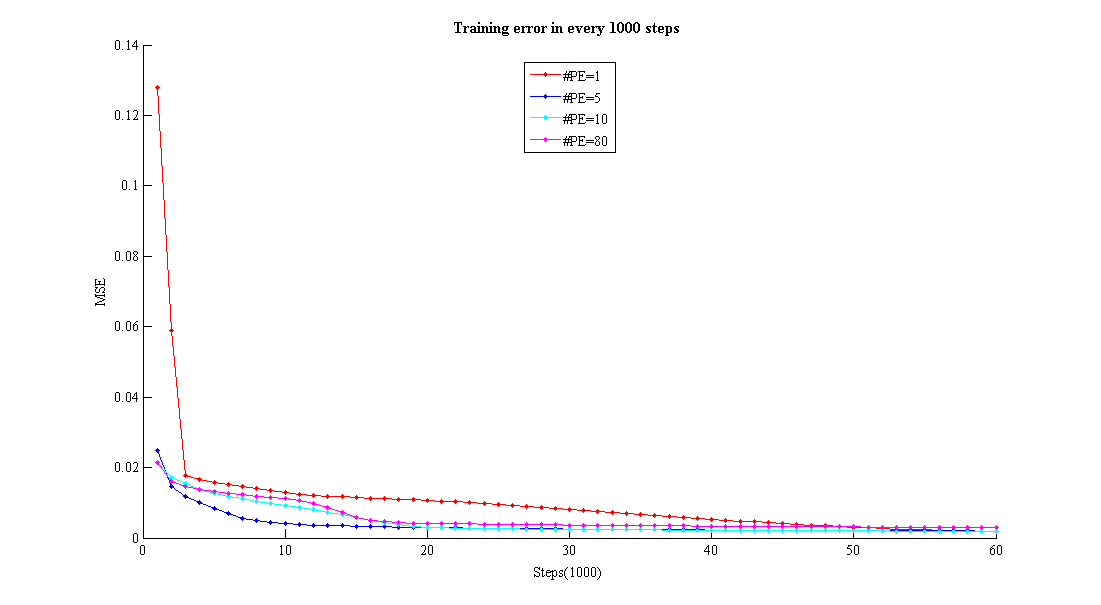
\includegraphics[width=6.5in]{errPE.png} 
\end{figure} 



{\bf 
\npar
2.1.2) Different learning rate 
\bpar
}

We used 0.01, 0.015 and 0.05 as learning rate. Interestingly, we found two patterns when learning rate is equal to 0.05. As shown below, the large learning rate can help the neuron network get to a small MSE much faster than the others and meet the criteria of stopping. The learning met the MSE less than or equal to the criteria at 27000 step. (Note that here we only showed the training error, no testing error).

\begin{figure}[H] 
\centering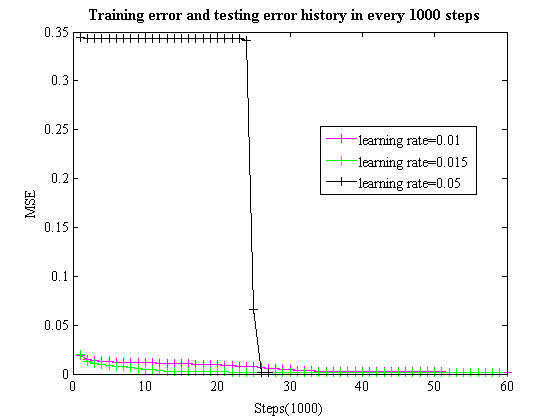
\includegraphics[width=4.5in]{lr_err1.png} 
\end{figure} 





However, in some other cases, using 0.05 as learning rate cannot converge the MSE, which is shown as figure below:

\begin{figure}[H] 
\centering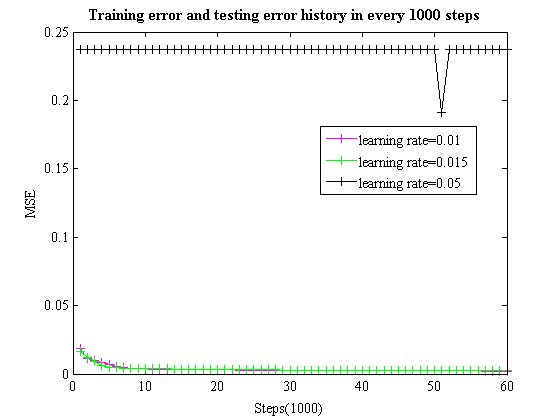
\includegraphics[width=4.5in]{lr_err2.png} 
\end{figure} 

And the learning failed.



{\bf 
\npar
2.2.1) Test the memory using $s_1{(n)}0.8sin({2\pi n \over 10}) + 0.25cos({2\pi n \over 25})$

\bpar
}

Test group 1: $s_1{(n)}0.8sin({2\pi n \over 10}) + 0.25cos({2\pi n \over 25})$

The MSE history is shown as below.

\begin{figure}[H] 
\centering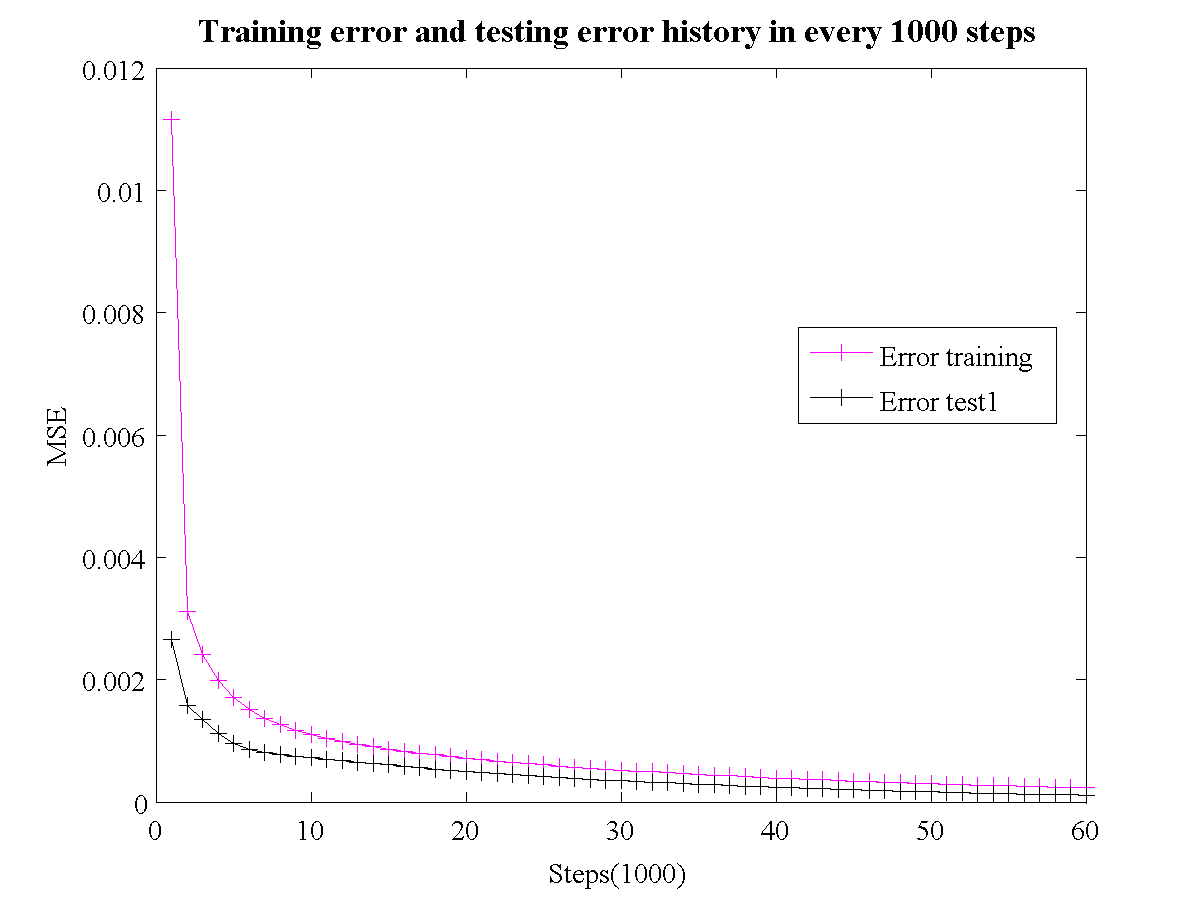
\includegraphics[width=4.5in]{err_test1.png} 
\end{figure} 

The training, testing output versus desired output is shown as figure below, where the final MSE is 0.0001 for testing, 0.0002 for training.

\begin{figure}[H] 
\centering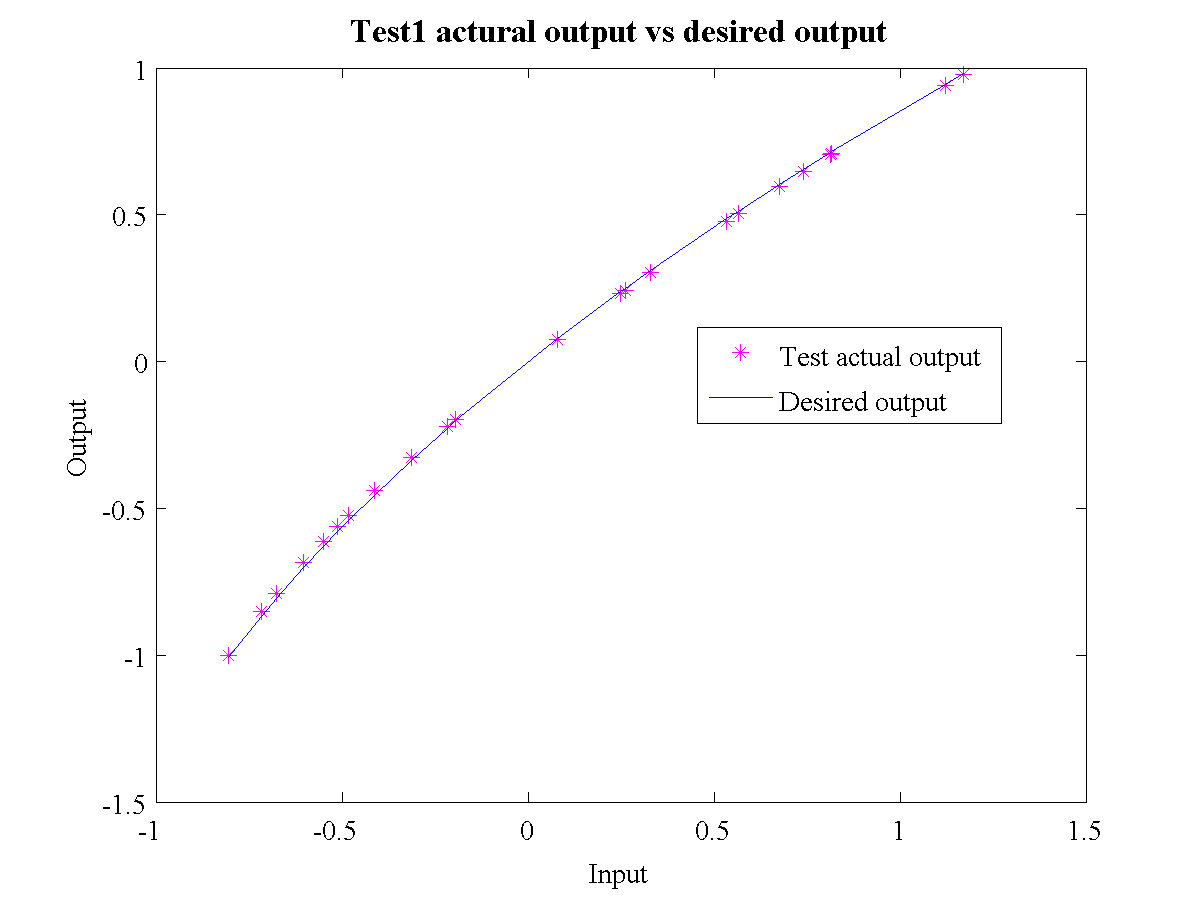
\includegraphics[width=4.5in]{output_test1.png} 
\end{figure} 




{\bf 
\npar
2.2.1) Test the memory using test group 2

\bpar
}


Test group 2: $s_2{(n)}$), 50 random numbers drawn from a zero mean, unit variance normal distribution.


The MSE history is shown as below.  The final MSE for testing group is 0.00021, for training group is 0.00023.

\begin{figure}[H] 
\centering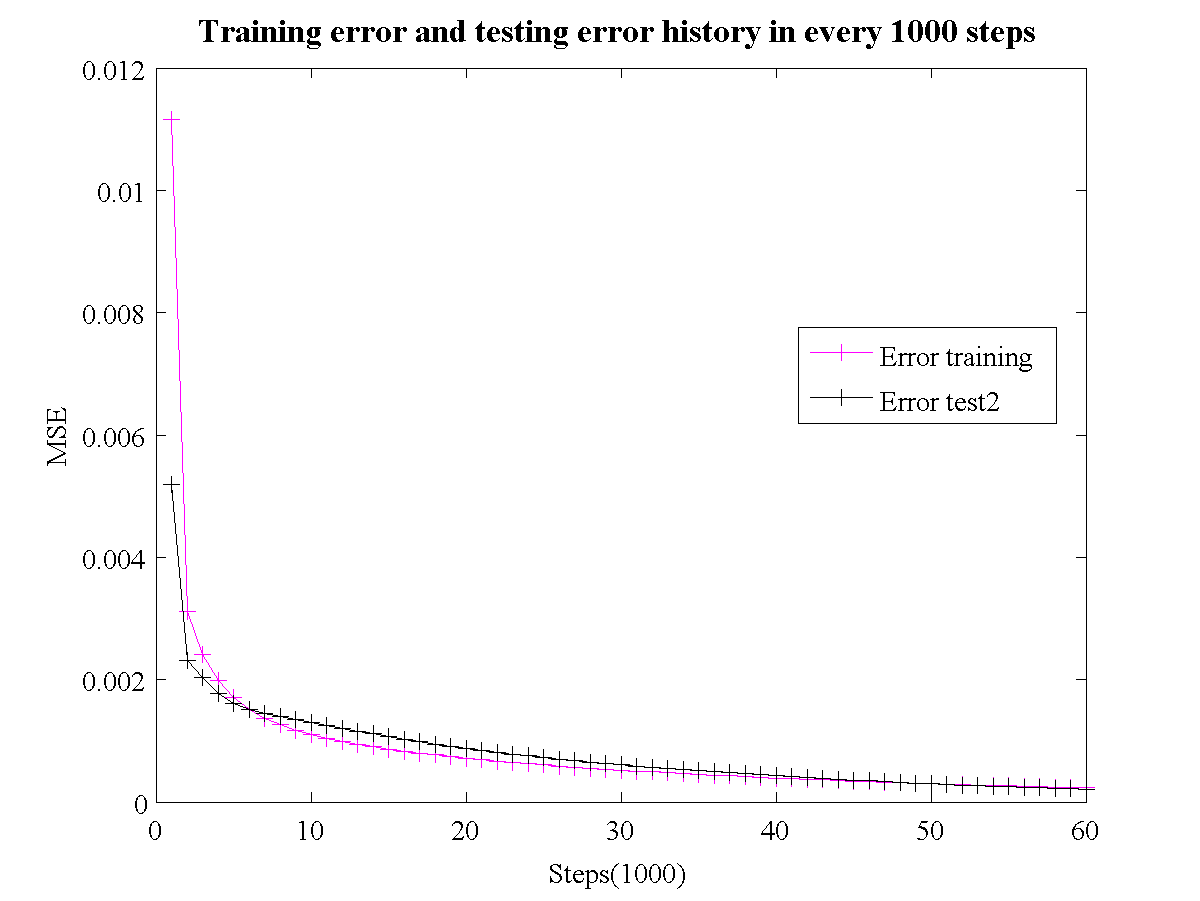
\includegraphics[width=4.5in]{err_test2.png} 
\end{figure} 

The training, testing output versus desired output is shown as figure below:

\begin{figure}[H] 
\centering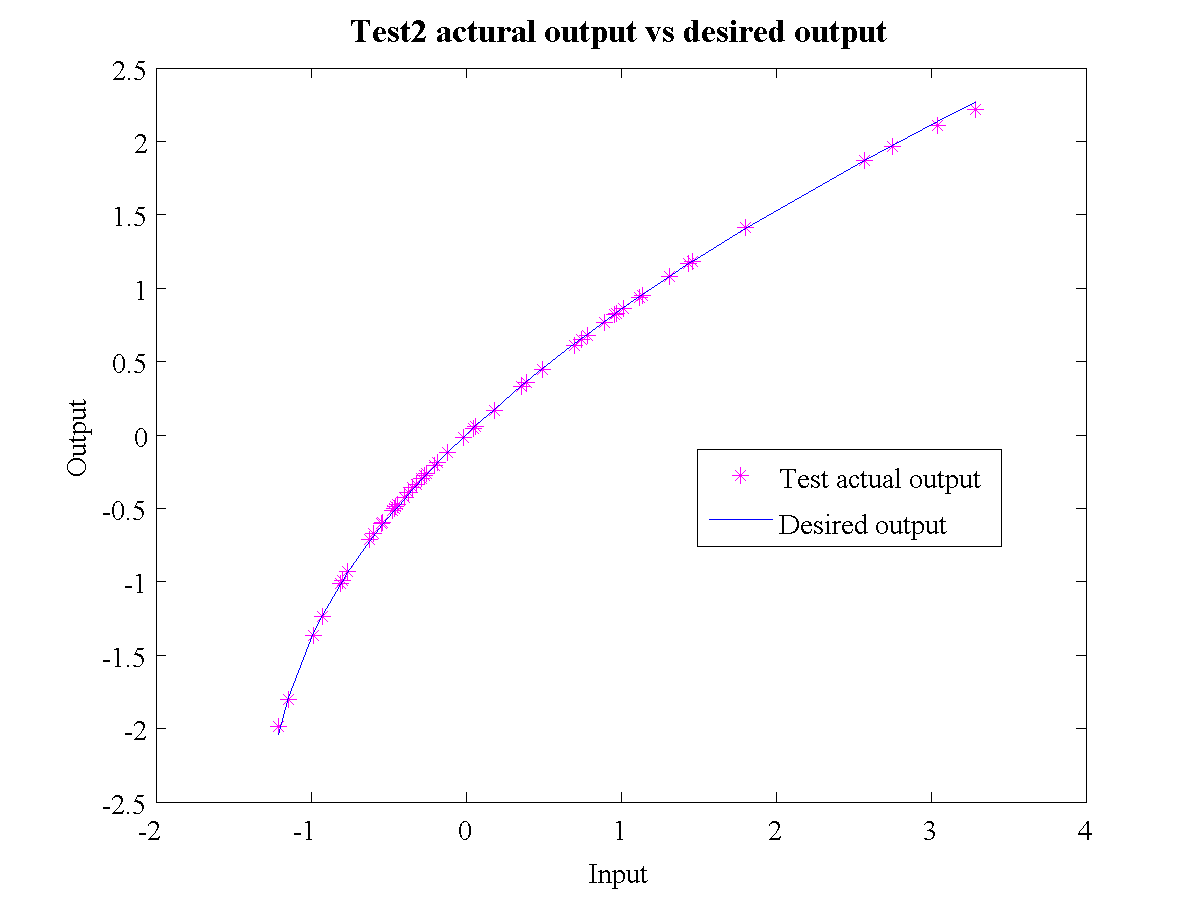
\includegraphics[width=4.5in]{output_test2.png} 
\end{figure} 

\end{document}